\documentclass[10pt, aspectratio=169, progressbar=frametitle]{beamer}
\usepackage{iftex}
\usetheme[numbering=none]{metropolis}
% \usetheme[language=en]{UniMS}

\setbeamertemplate{headline}{}

% \includeonlyframes{current}

\newcommand{\methodheader}{\multicolumn{1}{c}{\multirow{2}{*}{Method}}}

% Add table header (two-lines tall) with line breaks.
% #1 desired width (use em's please)
% #2 header's text (with line breaks via backslashes)
\newcommand{\headerWithBreaks}[2]{{%
\multirow{2}{*}{%
  \begin{minipage}[t]{#1}{#2}\end{minipage}
}
}}

% -----------------------------------------------------------------------------
% Fonts
\ifluatex
  \usepackage{unicode-math}
  \usepackage{fourier-otf}
  \setsansfont[BoldFont={Fira Sans SemiBold}]{Fira Sans Book}
  \setmonofont{Fira Code}
\else
\usepackage[defaultsans,scale=1.0]{lato}
\usepackage{fourier}
\usepackage[scale=1.05]{inconsolata}
\usefonttheme[onlymath]{serif}
\fi


% -----------------------------------------------------------------------------
% Typography
\usepackage{siunitx}
\usepackage{booktabs}
\usepackage{multirow}

% -----------------------------------------------------------------------------
% Graphics
\usepackage{pgfplots}
\usepackage{tikz}
\usepackage[beamer,customcolors]{hf-tikz}
\usetikzlibrary{arrows.meta, calc, positioning, shapes.geometric}
\usepackage[dvipsnames]{xcolor}
\usepackage{tikz}
\usetikzlibrary{arrows.meta, calc, positioning, shapes.geometric}

% General colors
\definecolor{MaRDI-blue}{RGB}{0,94,170}
\definecolor{MaRDI-orange}{RGB}{208,102,43}
\colorlet{MaRDI-grey}{black!40} % 40% black
\colorlet{MaRDI-gray}{MaRDI-grey}

% Light colors
\colorlet{MaRDI-light-blue}{MaRDI-blue!60}
\colorlet{MaRDI-blue-light}{MaRDI-light-blue}
\colorlet{MaRDI-lightest-blue}{MaRDI-blue!40}
\colorlet{MaRDI-blue-lightest}{MaRDI-lightest-blue}

\tikzset{%
  every path/.style={thick},
    edge/.style={%
        ->,
        >={Stealth[scale=1]},
    },
    usercode/.style={%
        rectangle,
        fill=MaRDI-orange,
        draw=black, thick,
        minimum width=3em,
        rounded corners=2pt,
        text=white,
        font=\footnotesize \sffamily,
        text centered,
    },
    lib/.style={%
        ellipse,
        fill=MaRDI-gray,
        minimum width=.12\linewidth,
        minimum height=.04\linewidth,
        rounded corners=2pt,
        text=white,
        font=\footnotesize \sffamily,
        text centered,
    },
    solver/.style={%
        rectangle,
        fill=MaRDI-blue,
        draw=black, thick, dashed,
        text=white,
        font=\footnotesize \sffamily,
        text centered,
        minimum width=3em,
        rounded corners=2pt,
    },
    grid/.style={%
      gray!20,
    }
}

\graphicspath{{./assets}{./tikz}}

% -----------------------------------------------------------------------------
% Define useful colors.
\colorlet{black}{black!50!gray}
\colorlet{green}{green!50!gray}
\colorlet{blue}{blue!50!gray}

\colorlet{CBlue}{blue!15}
\colorlet{CBlueD}{blue!95!gray}
\colorlet{CRed}{red!15}
\colorlet{CRedD}{red!65!gray}
\colorlet{CGreenD}{green!60!gray}
\colorlet{COrange}{orange}

\definecolor{CMaRDIBlue40}{RGB}{153, 191, 221}
\definecolor{CMaRDIOrange100}{RGB}{208, 102, 043}
\definecolor{CMaRDIOrange40}{RGB}{236, 194, 170}

% -----------------------------------------------------------------------------

\usepackage{derivative}
\usepackage{minted}

% -----------------------------------------------------------------------------
\setbeamersize{text margin left=0.5cm, text margin right=0.5cm}
\setbeamercolor{background canvas}{bg=white}
\setbeamercolor{frametitle}{fg=black, bg=white}
\setbeamercolor{title separator}{fg=CMaRDIOrange100, bg=CMaRDIOrange100}
\setbeamercolor{progress bar in section page}{fg=CMaRDIOrange100, bg=CMaRDIOrange40}

% -----------------------------------------------------------------------------
% Title info
\title{%
  The MaRDI Open Interfaces software project\\to improve interoperability in
  Scientific Computing}
\author{Dmitry I. Kabanov, Stephan Rave, Mario Ohlberger}
\institute{Mathematics Münster, University of Münster, Germany}
\date{Oberseminar Numerik, 29 October 2025}
\titlegraphic{\vspace{0.8\textheight}\hspace{0.38\textwidth}
  \includegraphics[width=0.618\textwidth]{logos/logos}
}

% -----------------------------------------------------------------------------
\begin{document}
\maketitle

\begin{frame}{Typical situation in scientific computing}
  \begin{itemize}
    \item Often computational scientists need
          to combine multiple solvers to conduct experiments
    \item They have a preferred language but some solvers are implemented
          not in this language
    \item For example, they prefer to conduct experiments using Python
          but a part of the experiment must use a solver written in C
    \item If the bindings to Python are not available, they need to write
          them themselves
    \item \dots Later, there's a need to replace the solver with
          another one $\implies$ code modification
    \item<2-> \alert{Two problems:} different languages and different interfaces
  \end{itemize}
\end{frame}

\begin{frame}{Traditional way: direct bindings}
  \begin{minipage}{0.45\textwidth}
    \begin{itemize}
      \item For a solver in C provide bindings to~$L$~languages: Python, Julia, R, \dots
      \item Repeat for a set of $I$ implementations of numerical algorithms
            and~$L$~languages
      \item It leads to $\mathcal O(L \times I)$ amount of work\\
      if we want to provide bindings\\
      for each algorithm in each language
    \end{itemize}
  \end{minipage}\hfill
  \begin{minipage}{0.45\textwidth}
    \centering
    \includegraphics{pairwise_bindings}
  \end{minipage}
\end{frame}

\begin{frame}[label=current]{Another solution}
  \begin{columns}[t]
    \column{0.5\textwidth - 2\tabcolsep}
    To solve both issues:
    \begin{itemize}
      \item \textbf{provide generic interfaces} for typical numerical problems,
            employing the software principle
            \emph{``program against an interface, not an implementation''}
      \item \textbf{automate data marshalling} between languages
            to avoid writing manual/semi-manual bindings
            (using tools like Cython, etc.)
    \end{itemize}

    \column{0.5\textwidth - 2\tabcolsep}
    \onslide<2->
    Examples of generic interfaces are:
    \begin{itemize}
      \item \texttt{BLAS} for basic linear algebra
      \item \texttt{scipy.optimize} in Python for optimization algorithms
      \item \texttt{OrdinaryDiffEqs.jl} in Julia for solving initial-value problems for ODEs
      \item \texttt{PyMOR} for model-order reduction simulations
    \end{itemize}

    However, the above packages concentrate on solving only
    the problem of different interfaces, not on the problem
    of data marshalling.
  \end{columns}
\end{frame}

\begin{frame}{MaRDI Open Interfaces (TA2 Measure 2)}
  \begin{minipage}{0.45\textwidth}
    To solve both problems simultaneously:
    \begin{itemize}
      \item Provide a mediator library \texttt{OIF} that:
            \begin{itemize}
              \item handles data marshalling between different languages
              \item provides a set of generic interfaces
                    for typical numerical problems
            \end{itemize}
      \item Each interface abstracts out the discrepancies
            of different implementations
      \item For $L$ languages and $I$ implementations leads to
            the $\mathcal O (I + L)$ amount of work
    \end{itemize}
  \end{minipage}\hfill%
  \begin{minipage}{0.50\textwidth}
    \centering
    \includegraphics{oif_bindings}
  \end{minipage}
\end{frame}

\section{Software details}

\begin{frame}{Software details: Components}
  \centering
  % \includegraphics[scale=0.09]{arch}
  \begin{minipage}{0.48\textwidth}
    \centering \textbf{User-facing components}
  \begin{itemize}
    \item \emph{Gateway} - a language-specific common interface
          to a particular numerical problem
    \item \emph{Converter} - a language-specific converter of data
          to intermediate C representation
    \item \emph{Dispatch} - a C library that takes the data in C representation,
          loads a Bridge and asks it to load an implementation and stores it
          in a table
  \end{itemize}
  \end{minipage}
  \begin{minipage}{0.48\textwidth}
    \centering \textbf{Implementation-facing components}
    \begin{itemize}
      \item \emph{Bridge} - a language-specific C library that converts data
            to native types and invokes implementation functions
      \item \emph{Interface} - a virtual component that has, in principle,
            the same interface as a \emph{Gateway}
      \item \emph{Adapter} - an adapter from implementation to the \emph{Interface}
      \item \emph{Implementation} - actual solver, outside of system's boundary
    \end{itemize}
  \end{minipage}
\end{frame}

\begin{frame}{Software details: Loading an implementation}
  \centering
  \includegraphics[scale=0.7]{uml-diagrams/impl_1_load}
\end{frame}

\begin{frame}{Software details: Calling an implementation}
  \centering
  \includegraphics[scale=0.7]{uml-diagrams/impl_2_call}
\end{frame}

\begin{frame}{Software details: Currently supported languages, data types, function calls}
  \begin{itemize}
    \onslide<1->
    \item Languages: C, Julia, and Python
    \onslide<2->
    \item Data types:
          \begin{itemize}
            \item \texttt{OIF\_INT} - 32-bit integers
            \item \texttt{OIF\_FLOAT64} - 64-bit floating-point numbers
            \item \texttt{OIF\_ARRAY\_F64} - arrays of 64-bit floating-point numbers
            \item \texttt{OIF\_STR} - strings
            \item \texttt{OIF\_CALLBACK} - callback functions
            \item \texttt{OIF\_USER\_DATA} - user-data objects of volatile type
            \item \texttt{OIF\_CONFIG\_DICT} - option-value pairs
          \end{itemize}
    \onslide<3->
    % \item Interfaces:
    %       \begin{itemize}
    %         \item (Toy test problem) quadratic equations: $ax^2 + bx + c = 0$
    %         % \item systems of linear algebraic equations: $Ax = b$
    %         \item initial-value problems for ODEs \(y'(t) = f(t, y), \  y(t_0) = y_0\)
    %       \end{itemize}
    \item On implementation side function are invoked via
          the Foreign Function Interface library \texttt{libffi}\footnote{\url{https://sourceware.org/libffi/}}
          in C and via C API in embedded Python/Julia
  \end{itemize}
\end{frame}


\begin{frame}{Software details: Special data structures for C}
  \small Package provides special data structures in C to ensure consistency
  with Julia and Python interfaces:
  \begin{itemize}
    \item \texttt{OIFArrayF64} packs array data along with shape\\
          \texttt{OIFArrayF64 *oif\_create\_array\_f64(int nd, intptr\_t *dimensions)}\\
          \texttt{OIFArrayF64 *oif\_init\_array\_f64\_from\_data(nd, dimensions, const double *data)
}
      \item<2-> \texttt{OIFConfigDict} packs key-value pairs together\\
          \texttt{void oif\_config\_dict\_add\_int(OIFConfigDict *dict, const char *key, int value);}\\
          \texttt{void oif\_config\_dict\_add\_double(OIFConfigDict *dict, const char *key, double value);}\\
          \texttt{void oif\_config\_dict\_add\_str(OIFConfigDict *dict, const char *key, const char *value);}
  \end{itemize}
\end{frame}

\begin{frame}{Software details: Passing arrays does not incur memory copies}
  \centering
  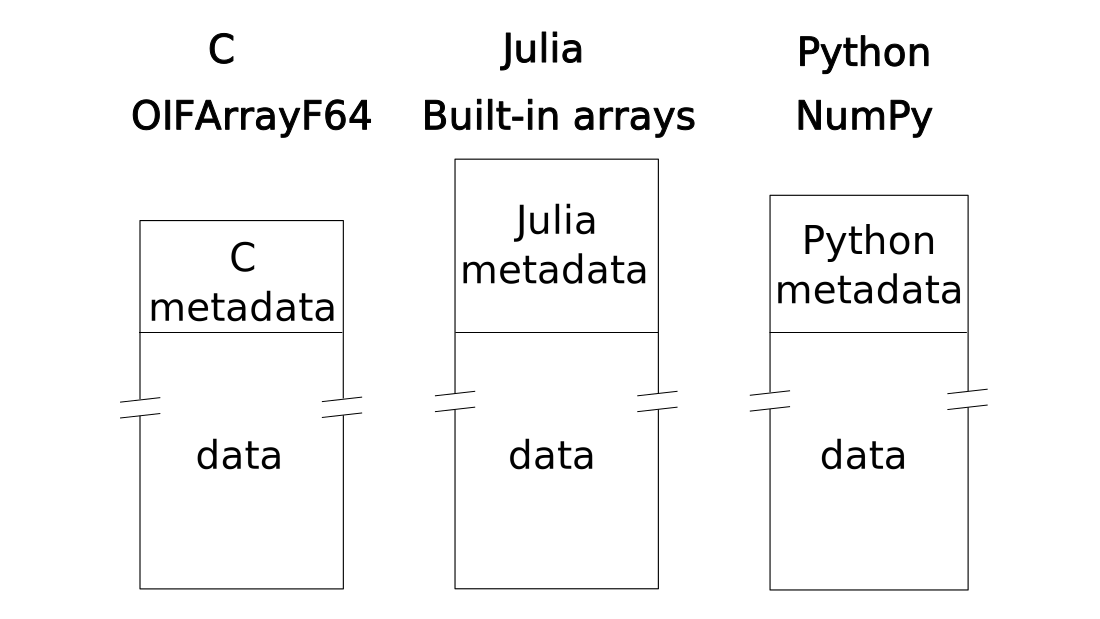
\includegraphics[scale=0.1]{arrays}

  Arrays are essentially just ``repacked'' for a particular language
  with metadata without copying array elements, which costs $\mathcal O(1)$.
\end{frame}

\section{Examples with the interface for initial-value problems for ODEs (time integration)}

\begin{frame}[fragile]{Interface for initial-value problems for ODEs}
  \begin{minipage}{\dimexpr0.22\textwidth-2\tabcolsep}
    \begin{align*}
      y'(t)  & = f(t, y) \\
      y(t_0) & = y_0
    \end{align*}
  \end{minipage}
  \begin{minipage}{\dimexpr0.73\textwidth-2\tabcolsep}
    {\footnotesize
    \begin{minted}{Python}
      # Set initial value y(t0) = y0.
      set_initial_value(y0: array, t0: float64)

      # Specify right-hand side function with signature
      # f(t: float64, y: array, ydot: array, user_data: object).
      set_rhs_fn(f: Callback)

      # Specify relative and absolute tolerances.
      set_tolerances(rtol: float64, atol: float64)

      # Set additional data passed to right-hand side function.
      set_user_data(user_data: object)

      # Set integrator and its parameters
      set_integrator(integrator_name: str, params: object)

      # Integrate to time t and write solution to y.
      integrate(t: float64, y: array)
    \end{minted}
    }
  \end{minipage}
\end{frame}

\begin{frame}[fragile]{Example 1: Exponential decay from C}
  \begin{columns}
    \column{0.3\textwidth}
  \begin{align*}
    \frac{\mathrm d y}{\mathrm d t} &= -y\\
    y(0) &= 1
  \end{align*}
  \vspace{-2em}
  \onslide<2>
  \begin{minted}[beameroverlays, escapeinside=||]{C}
int rhs(
  double t,
  OIFArrayF64 *y,
  OIFArrayF64 *rhs_out,
  void *user_data)
{
  for (
    int i = 0;
    i < y->dimensions[0]; ++i) {
      rhs_out->data[i] = -y->data[i];
  }
  return 0;
}
\end{minted}
  \column{0.7\textwidth}
  \onslide<3->
  \begin{minted}[beameroverlays, escapeinside=||]{C}
    char *|\textbf<4>{impl\_name}| = <implementation-string>;
    OIFArrayF64 *|\textbf<6>{y0}| = oif_create_array_f64(
      1, (intptr_t[1]){N});
    |\textbf<6>{y0}|->data[0] = 1.0;
    OIFArrayF64 *|\textbf<8>{y}| = oif_create_array_f64(
      1, (intptr_t[1]){N});

    ImplHandle |\textbf<5>{implh}| = oif_init_impl(
      "ivp", |\textbf<4>{impl\_name}|, 1, 0);
    status = oif_ivp_set_initial_value(|\textbf<5>{implh}|, |\textbf<6>{\{y0\}}|, |\textbf<6>{0.0}|);
    status = oif_ivp_set_rhs_fn(|\textbf<5>{implh}|, |\textbf<7>{rhs}|);

    for (int i = 0; i < n_time_steps; ++i) {
        t = t0 + (i + 1) * dt;
        status = oif_ivp_integrate(|\textbf<5>{implh}|, t, |\textbf<8>{y}|);
    }
  \end{minted}
  \end{columns}
\end{frame}

\begin{frame}[fragile]{Example 2: Solving a stiff system}
  \begin{columns}[t]
  \column{\dimexpr 0.4\textwidth - 2\tabcolsep}
    Van der Pol equation:
    \[
      \frac{\mathrm{d} x}{\mathrm{d} t} - \mu
      \left(
        1 - x^{2}
      \right) \frac{\mathrm{d} x}{\mathrm{d} t} + x = 0
    \]
    \(x(0) = 2\), \(t \in [0; 3000]\) and \(\mu = 1000\).\par

    \onslide<2>
    \vspace{3em}
    Transformed to a first-order system:
    \begin{align*}
      \frac{\mathrm{d} y_{0}}{\mathrm{d} t} &= y_{1}\\
      \frac{\mathrm{d} y_{1}}{\mathrm{d} t} &= \mu (1 - y_{0}^{2}) y_{1} - y_{0} \\
      y_{0}(0) &= 2, \quad y_{1}(0) = 0
    \end{align*}

    \vspace{5em}
    \onslide<3->
    \begin{tikzpicture}[overlay, remember picture]
      \node at (3, 4) {\includegraphics[width=0.99\textwidth]{ivp-vdp}};
    \end{tikzpicture}
  \column{0.6\textwidth - 2\tabcolsep}%
    \onslide<4->
    User code in Python:
    \begin{minted}[autogobble, beameroverlays, escapeinside=||]{Python}
    class VdPEquationProblem:
      ...
      def compute_rhs(self, __, y, ydot, ___):
          ydot[0] = y[1]
          ydot[1] = self.mu*(1-y[0]**2)*y[1]-y[0]
          return 0

      problem = VdPEquationProblem(mu=1000, T=3000)

      s = IVP(<impl-name>)
      # Optional step
      s.set_integrator(<name>, <options>)
      s.set_initial_value(problem.y0, problem.t0)
      s.set_rhs_fn(problem.compute_rhs)
    \end{minted}
  \end{columns}
\end{frame}

\begin{frame}[fragile]{Example 2: Solving a stiff system}
    \onslide<1->
    \begin{columns}
    \column{\dimexpr 0.6\textwidth - 2\tabcolsep}
      \begin{minted}[autogobble, beameroverlays, escapeinside=||]{Python}
        s = IVP("scipy_ode")
        s.set_integrator("dopri5", {"nsteps": 100_000})
      \end{minted}
    \column{\dimexpr 0.4\textwidth - 2\tabcolsep}
      \onslide<2->{%
      \textbf{\color{CRedD}Fail}\\
      \texttt{UserWarning: dopri5: problem is probably stiff}
      }
    \end{columns}

    \vspace{3em}
    \onslide<3->
    \begin{columns}
      \column{0.6\textwidth - 2\tabcolsep}
        \begin{minted}[autogobble, beameroverlays, escapeinside=||]{Python}
          s = IVP("scipy_ode")
          s.set_integrator("vode", {"nsteps": 40_000})
        \end{minted}

      \column{0.4\textwidth - 2\tabcolsep}
        \onslide<4->{%
        \textbf{\color{CGreenD}Success}\\
        However, time-to-solution is about 10 seconds.
        }
    \end{columns}

    \vspace{3em}
    \onslide<5->
    \begin{columns}
      \column{0.6\textwidth - 2\tabcolsep}
        \begin{minted}[autogobble, beameroverlays, escapeinside=||]{Python}
          s = IVP("jl_diffeq")
          s.set_integrator("Rosenbrock23")
          s.set_initial_value(problem.y0, problem.t0)
          s.set_rhs_fn(problem.compute_rhs)
        \end{minted}
      \column{0.4\textwidth - 2\tabcolsep}
        \onslide<6->{%
          \textbf{\color{CGreenD}Success}\\
          More efficient solution using \texttt{OrdinaryDiffEq.jl}
        }
    \end{columns}
\end{frame}

\section{Runtime performance}

% \begin{frame}{Performance study}
%   We solve a 2D Gray--Scott reaction-diffusion system\footnote{Pearson, J.\ E.
%     \emph{Complex Patterns in a Simple System}, 1993, doi:
%     \href{https://doi.org/10.1126/science.261.5118.189}{%
%       10.1126/science.261.5118.189}}:
%   \begin{align*}\label{eq:gs-system}
%     \begin{split}
%       \frac{\partial u}{\partial t} &= d_u \nabla^2 u - u v^2 + F (1 - u), \\
%       \frac{\partial v}{\partial t} &= d_v \nabla^2 v + u v^2 - (F + k) v
%     \end{split}
%   \end{align*}
%   with periodic boundary conditions on the domain $[-2.5; 2.5]^2$ with initial
%   condition given by \(u = 1\), \(v = 0\) everywhere in the domain, except
%   a square of \(40 \times 40\) grid points  centered in the center of the domain,
%   which is set to \(u = 0.5 + \mathrm{Uniform}(0; 0.1)\)
%   and \(v = 0.25 + \mathrm{Uniform}(0; 0.1)\).

%   Final time 100 with time step 1.
%   Parameters \(F = 0.055\), \(k = 0.062\), \(d_u = \num{2e-5}\),
%   \(d_v = \num{e-5}\).
% \end{frame}

% \begin{frame}{Performance study, cont.}
%   \begin{minipage}{0.48\textwidth}
%     Resolution \(N \in \{64, 128, 256, 512\}\)\\
%     For each \(N\) three runs\\
%     User code is in Python\\
%     Implementation code is in C (Sundials CVODE\footnotemark)

%     \vspace{6em}
%     Normalized runtime of the Sundials CVODE solver via Open Interfaces
%     vs direct bindings using the~\texttt{scikit.odes}\footnotemark\
%     software package.
%   \end{minipage}\hfill
%   \begin{minipage}{0.48\textwidth}
%     \centering
%     \includegraphics[scale=0.45]{ivp_cvode_gs_performance}
%   \end{minipage}
%   \footnotetext{%
%     Hindmarsh, A.\ C. et al. \emph{SUNDIALS: Suite of Nonlinear and Differential/Algebraic Equation Solvers}, 2005%, doi:
%     %\href{https://doi.org/10.1145/1089014.1089020}{10.1145/1089014.1089020}
%   }
%   \footnotetext{%
%     Benny, P.\ K., et al. \emph{bmcage/odes: Release 2.7.0}, 2023, doi:
%     \href{https://doi.org/10.5281/ZENODO.7533040}{10.5281/ZENODO.7533040}
%   }
% \end{frame}

\begin{frame}{Performance study}
  \begin{minipage}{\dimexpr0.6\textwidth - 2\tabcolsep}
  We solve inviscid Burgers' equation
    \begin{align*}
      &\pdv{u}{t} + \pdv{\left( u^{2} / 2 \right)}{x} = 0,
      \quad t \in [0, 2], \quad x \in [0, 2] \\
      &u(t, 0) = 0.5 - 0.25 \sin \left( \pi x \right)\\
      &u(t, 0) = u(t, 2)
    \end{align*}
  using implementations of the Dormand--Prince Runge--Kutta 5(4) method:
  \begin{itemize}
  \item C: reimplemented from the original Fortran code\footnote{%
  Hairer E., Wanner, G., Nørsett, S.\ P. 
  \emph{Solving Ordinary Differential Equations I: Nonstiff Problems}, 1993}
  \item Julia: OrdinaryDiffEq.jl\footnote{%
          \url{https://github.com/SciML/OrdinaryDiffEq.jl}} \texttt{DP5}
  \item Python: SciPy\footnote{\url{https://scipy.org/}} \texttt{dopri5}
  \end{itemize}
  \end{minipage}\hfill
  \begin{minipage}{\dimexpr0.4\textwidth - 2\tabcolsep}
    % \includegraphics[width=0.9\textwidth]{ivp_c_burgers_eq}
    \includegraphics[width=0.9\textwidth]{ivp-burgers}
  \end{minipage}
\end{frame}

\begin{frame}
  \frametitle{Performance study: right-hand side implementations}

  \centering
  Runtimes of only right-hand side functions
  evaluated 10\,000 times at $N=6\,400$
  \vspace{1em}

  \begin{tabular}{l c}
    \toprule
    Implementation language & Runtime, seconds \\
    \midrule
    C (Clang)               & 0.115 \(\pm\) 0.008    \\
    Julia                   & 0.122 \(\pm\) 0.016    \\
    Python (Numba)          & 0.116 \(\pm\) 0.001    \\
    \bottomrule
  \end{tabular}
\end{frame}

\begin{frame}
  \frametitle{Performance study: results}

\newcommand{\myheader}{%
\headerWithBreaks{0.2em}{\#} &
\headerWithBreaks{3em}{User\\language} &
\headerWithBreaks{1.5em}{OIF/\\RAW} &
\headerWithBreaks{3em}{Imple-\\mentation} &
                                \multicolumn{2}{c}{$N$} \\
                                \cmidrule(lr){5-6}
}
  \vspace{1em}
  \centering
  \begin{tabular}{l l l l c c}
    \toprule
    \myheader                                                                                    \\
                       &           &     &          & 6400                & 25\,600              \\
    \midrule
    \multirow{2}{*}{1} & C         & OIF & DOPRI5-C & 1.011 \(\pm\) 0.017 & 21.006 \(\pm\) 0.100 \\
                       & C         & RAW & DOPRI5-C & 0.951 \(\pm\) 0.012 & 20.699 \(\pm\) 0.121 \\
    \addlinespace
    \addlinespace
    \multirow{3}{*}{2} & C         & OIF & DP5      & 0.847 \(\pm\) 0.003 & 20.700 \(\pm\) 0.049 \\
                       & Julia (C) & RAW & DP5      & 0.820 \(\pm\) 0.008 & 20.364 \(\pm\) 0.073 \\
                       & Julia     & RAW & DP5      & 0.868 \(\pm\) 0.004 & 21.058 \(\pm\) 0.067 \\
    \addlinespace
    \addlinespace
    \multirow{3}{*}{3} & Python    & RAW & DOPRI5   & 1.573 \(\pm\) 0.010 & 30.829 \(\pm\) 0.121 \\
                       & Python    & OIF & DOPRI5   & 1.575 \(\pm\) 0.005 & 30.944 \(\pm\) 0.122 \\
                       & Python    & OIF & DP5      & 1.466 \(\pm\) 0.005 & 28.147 \(\pm\) 0.040 \\
    \bottomrule
  \end{tabular}
\end{frame}

% \begin{frame}{MaRDI}
  \begin{itemize}
    \item This project is part of MaRDI---Mathematical Research Data Initiative.
    \item The overall goal of MaRDI is to improve infrastructure related
          to mathematics and other scientific dispiplines
    \item Points of interests are data formats, FAIRness of data
          (Findable, Accessible, Interoperable, Reproducable), computational
          workflows
  \end{itemize}
  \vspace{-2cm}
  \includegraphics[scale=0.7]{MaRDI_Logo_S_5_cmyk}
\end{frame}


\begin{frame}
  \begin{minipage}{0.618\textwidth}
    \begin{itemize}
      \item Open source, BSD-2-Clause License
      \item \url{https://github.com/MaRDI4NFDI/open-interfaces}
      \item Preprint: \url{https://arxiv.org/abs/2504.03628}
    \end{itemize}
  \end{minipage}%
  \begin{minipage}{0.382\textwidth}
    \includegraphics[scale=0.2]{github}
  \end{minipage}
\end{frame}

\begin{frame}
  \centering
  \vspace{9em}
  \huge{Thank you!}

  \vspace{3em}
  \includegraphics[width=0.618\linewidth]{logos/logos}
\end{frame}
\end{document}
